\chapter{Resultados}

Neste capítulo serão apresentados os resultados preliminares, provenientes dos testes realizados bem como refinamento da ferramenta e seus parâmetros, a sessão 4.1 apresentará os resultados obtidos com o PhotoGuide; na sessão 4.2 os resultados preliminares com o \textit{LSD-SLAM} serão mostrados. A seção 4.3 trará os problemas encontrados.

\section{Resultados com o PhotoGuide}

Primeiramente o aplicativo operou sem usar nenhuma das três formas de filtragem descritas anteriormente, ocasionando num grande número de falsos casamentos, como apresentam as imagens \ref{fig4:1} e \ref{fig4:2}:

\begin{figure}[!htb]
	\centering
		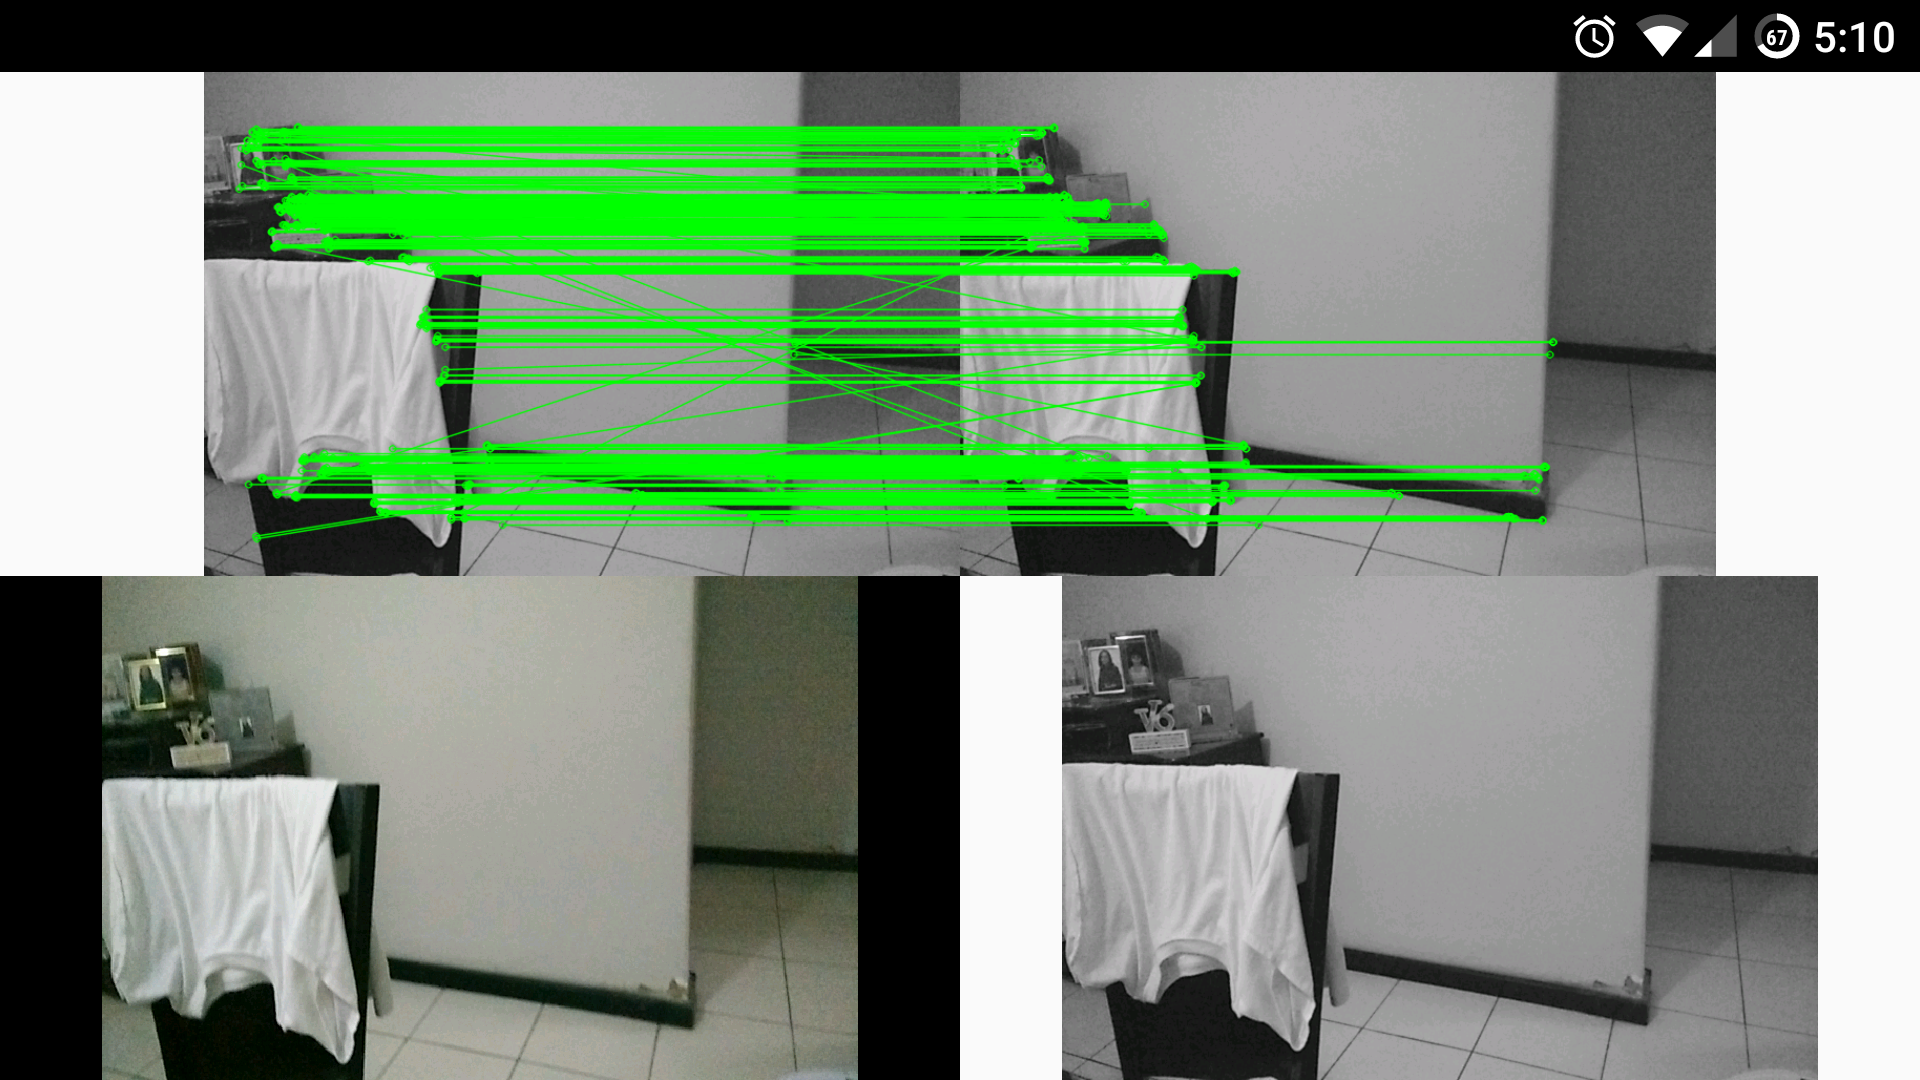
\includegraphics[width= \textwidth]{Imagens/figura4-1.png}
	\caption{Exemplo de execução do PhotoGuide sem nenhuma filtragem de casamentos}
	\label{fig4:1}
\end{figure}

\begin{figure}[!htb]
	\centering
		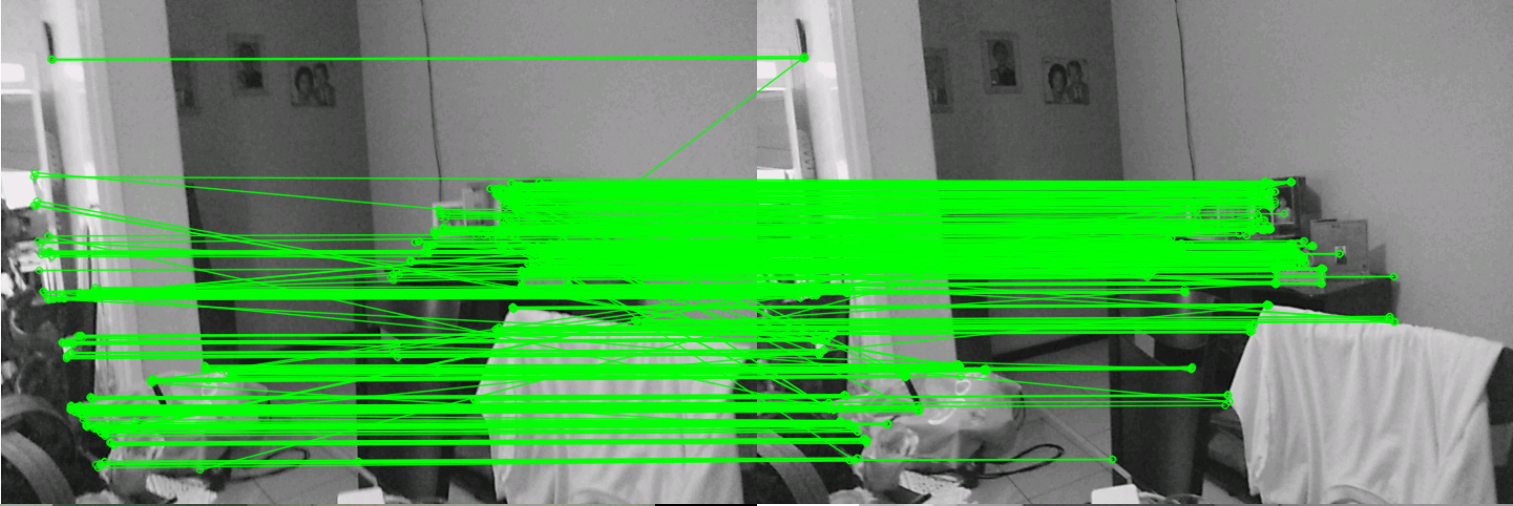
\includegraphics[width= \textwidth]{Imagens/figura4-2.png}
	\caption{Segundo exemplo de execução do PhotoGuide sem nenhuma filtragem de casamentos}
	\label{fig4:2}
\end{figure}

Essa situação é pior quando o ambiente possui partes em vidro, como mesas ou janelas, dificultando ainda mais a casamento de pontos, como mostra a figura \ref{fig4:3}

\begin{figure}[!htb]
	\centering
		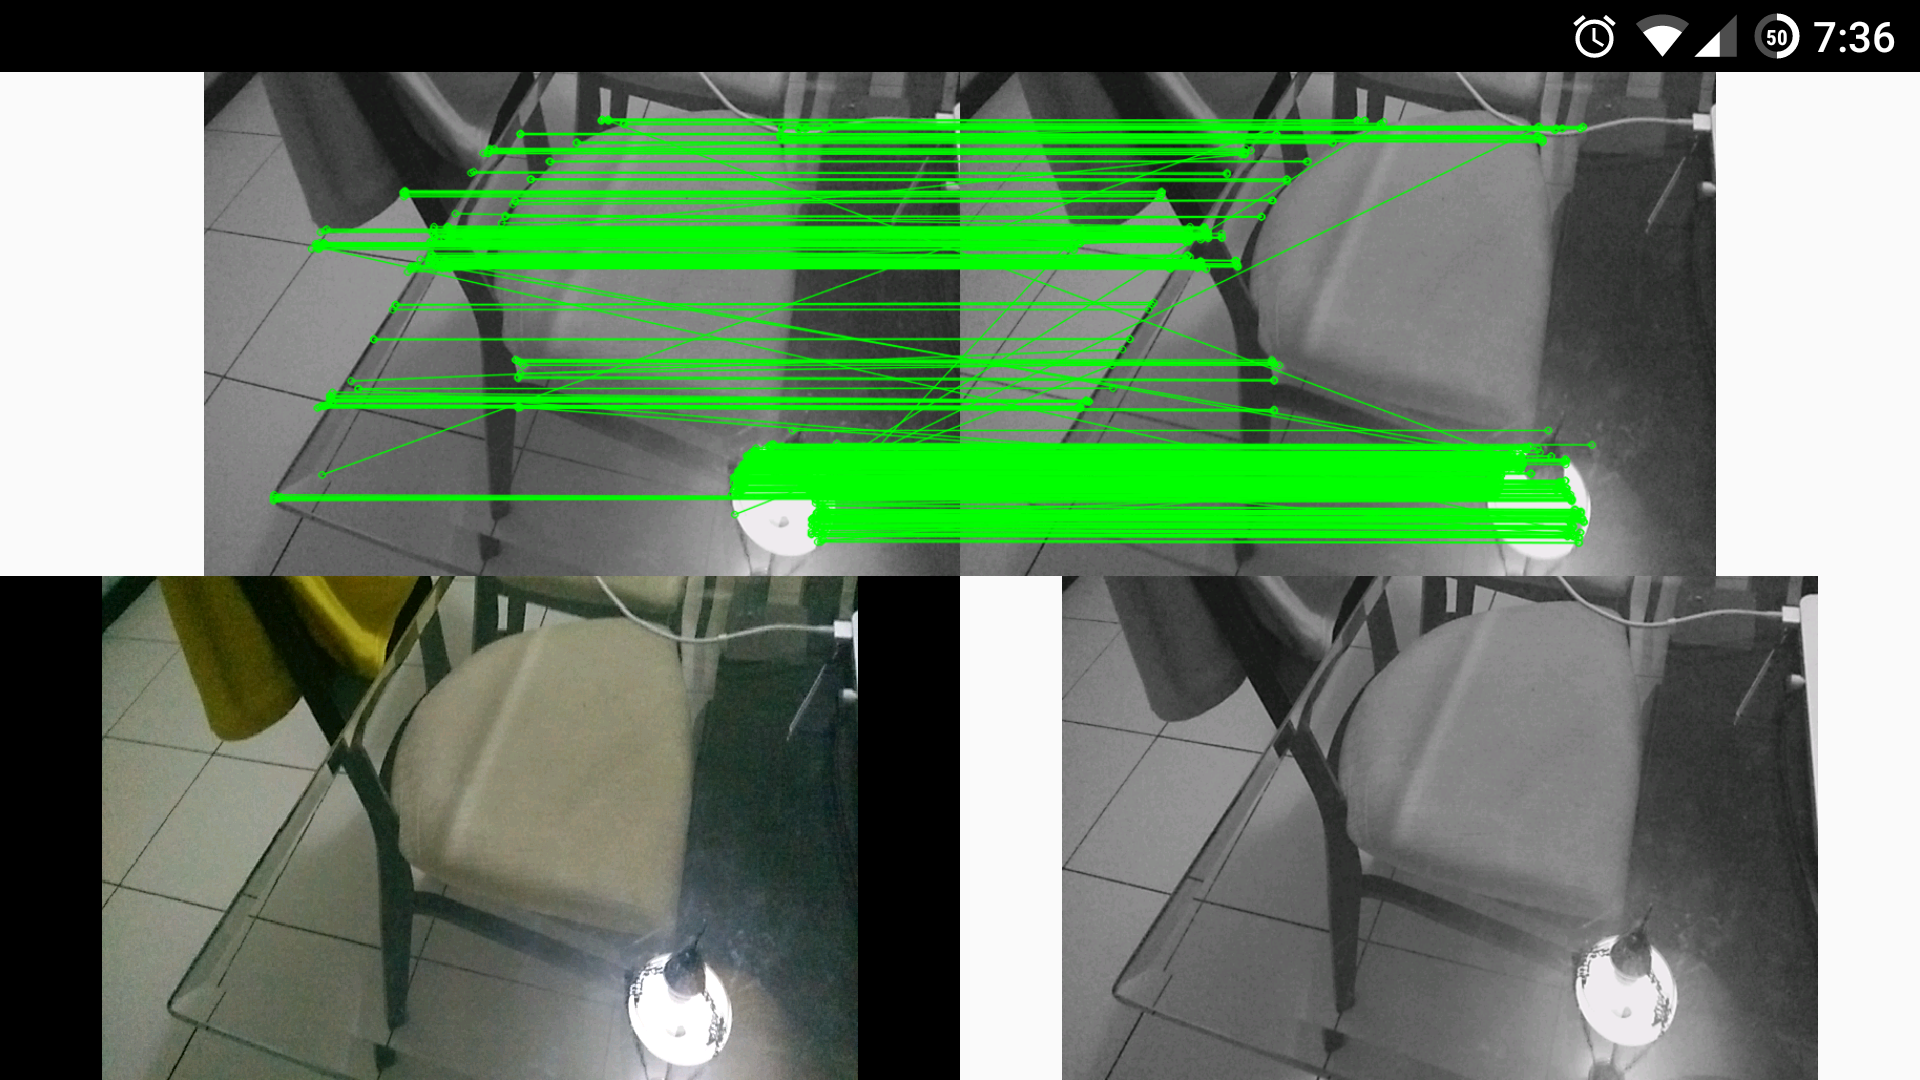
\includegraphics[width= \textwidth]{Imagens/figura4-3.png}
	\caption{Exemplo de execução do PhotoGuide sem nenhuma filtragem de casamentos e com peças em vidro, dificultando os casamentos}
	\label{fig4:3}
\end{figure}

Ao se adicionar os métodos de filtragem explicados na seção 3.1, é possível eliminar diversos casamentos errôneos, como na figura \ref{fig4:4}:

\begin{figure}[!htb]
	\centering
		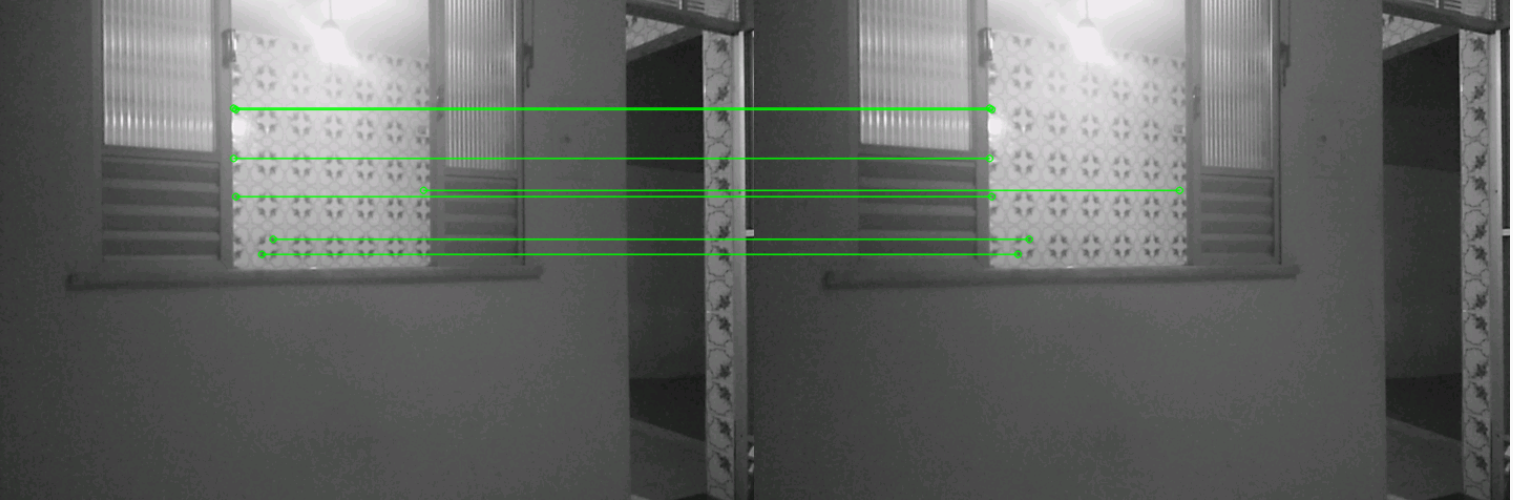
\includegraphics[width= \textwidth]{Imagens/figura3-2E4-4.png}
	\caption{Exemplo da filtragem de casamentos}
	\label{fig4:4}
\end{figure}

Infelizmente, dependendo do ambiente, o número de casamentos pode ser muito pequeno para se tornar significativo para a reconstrução 3D. Foram realizados testes diminuindo a sensibilidade com qual os casamentos eram filtrados, ou a não execução de alguma filtragem, mas ainda eram encontrados falso positivos, sendo necessário todos os métodos de filtragem. 
	Tendo em vista os problemas com o desempenho no aparelho utilizado, bem como problemas com o algoritmo, a continuação do trabalho se deu com a ferramenta \textit{LSD-SLAM}, e a funcionalidade de calibração e exportação de arquivo de calibração do PhotoGuide foi útil para utilizar a calibração de smartphones em testes com o \textit{LSD-SLAM}, bem como a possibilidade de trabalhos futuros onde seja desejado exportar a calibração da câmera ou obter datasets partindo do \textit{smartphone}.
	
\section{Resultados com o \textit{LSD-SLAM}}

O \textit{LSD-SLAM} possui diversos parâmetros que podem auxiliar na visualização e refinamento de como seus algoritmos funcionam. Os testes preliminares foram realizados em um dos laboratórios do DCOMP, mais precisamente, o laboratório de mestrado II, na área externa do prédio e também em um quintal, este último para testar os resultados sob um ambiente com mais texturas e menos homogêneo. As figuras \ref{fig4:5} a \ref{fig4:15} mostram as \textit{pointclouds} obtidas e fotografias dos ambientes:

\begin{figure}[!htb]
	\centering
		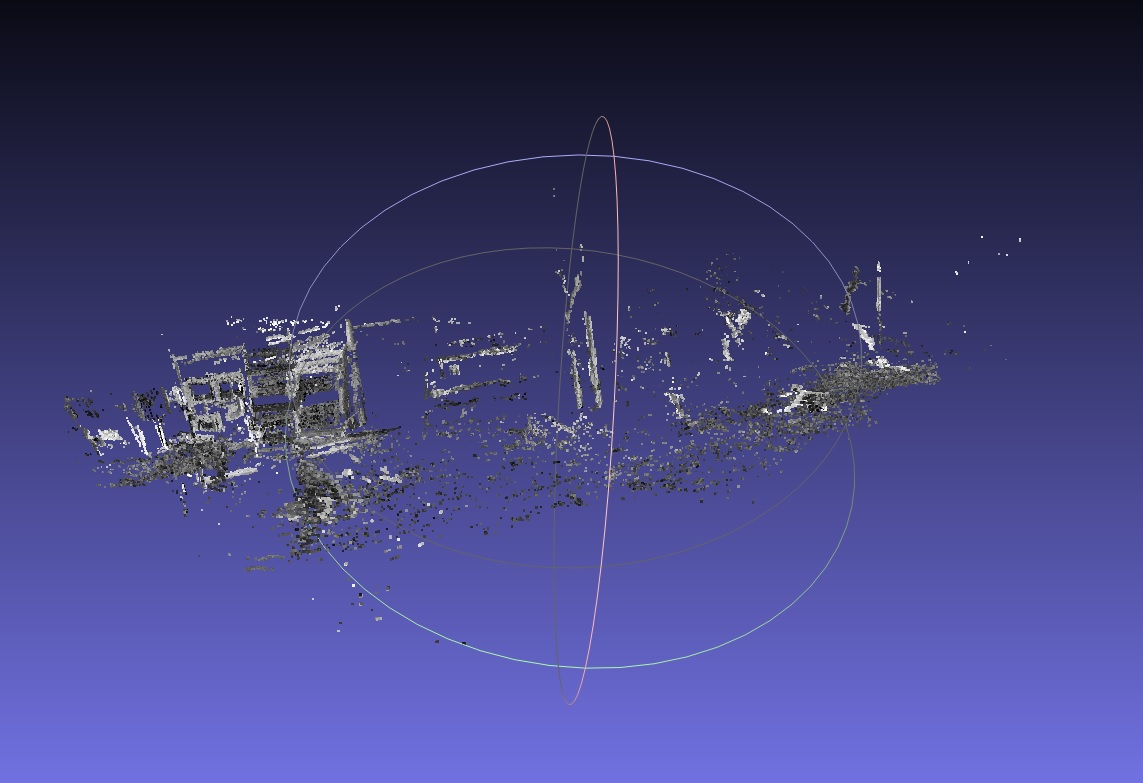
\includegraphics[width= \textwidth]{Imagens/figura4-5.jpg}
	\caption{Exemplo do \textit{pointcloud} da área externa do DCOMP \#1}
	\label{fig4:5}
\end{figure}

\begin{figure}[!htb]
	\centering
		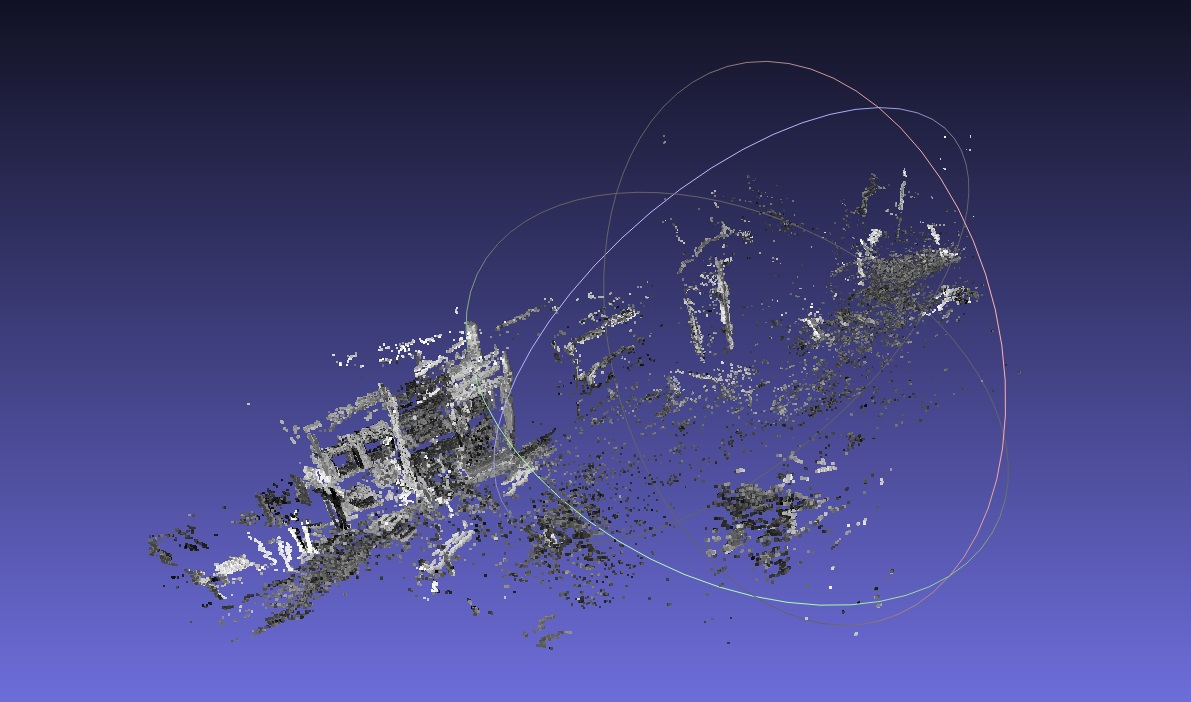
\includegraphics[width= \textwidth]{Imagens/figura4-6.jpg}
	\caption{Exemplo do \textit{pointcloud} da área externa do DCOMP \#2}
	\label{fig4:6}
\end{figure}

\begin{figure}[!htb]
	\centering
		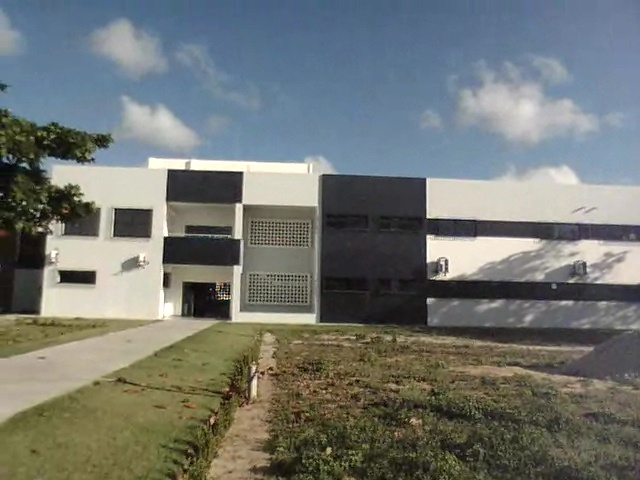
\includegraphics[width= \textwidth]{Imagens/figura4-7.jpg}
	\caption{Fotografia da área mapeada}
	\label{fig4:7}
\end{figure}

\begin{figure}[!htb]
	\centering
		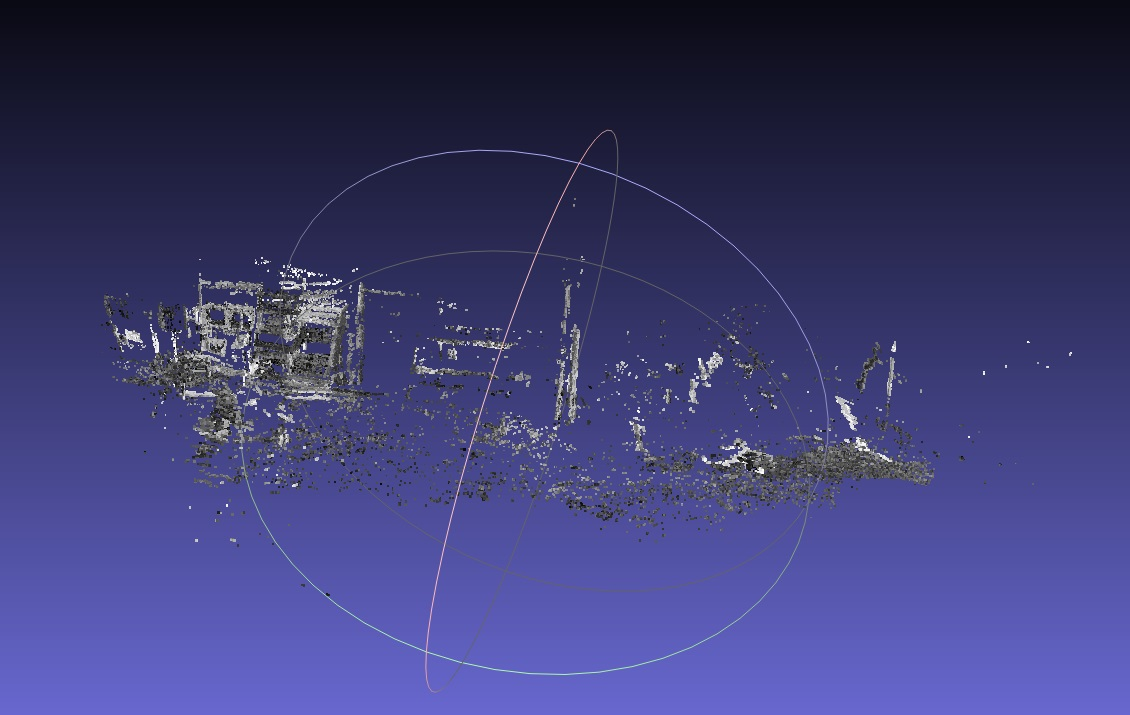
\includegraphics[width= \textwidth]{Imagens/figura4-8.jpg}
	\caption{Outro \textit{pointcloud} da área externa do DCOMP, sob outro ângulo}
	\label{fig4:8}
\end{figure}

\begin{figure}[!htb]
	\centering
		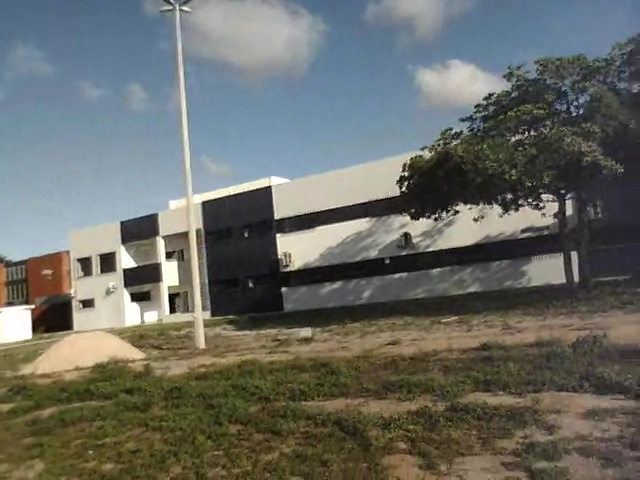
\includegraphics[width= \textwidth]{Imagens/figura4-9.jpg}
	\caption{\textit{Pointcloud} da figura \ref{fig4:8}}
	\label{fig4:9}
\end{figure}

\begin{figure}[!htb]
	\centering
		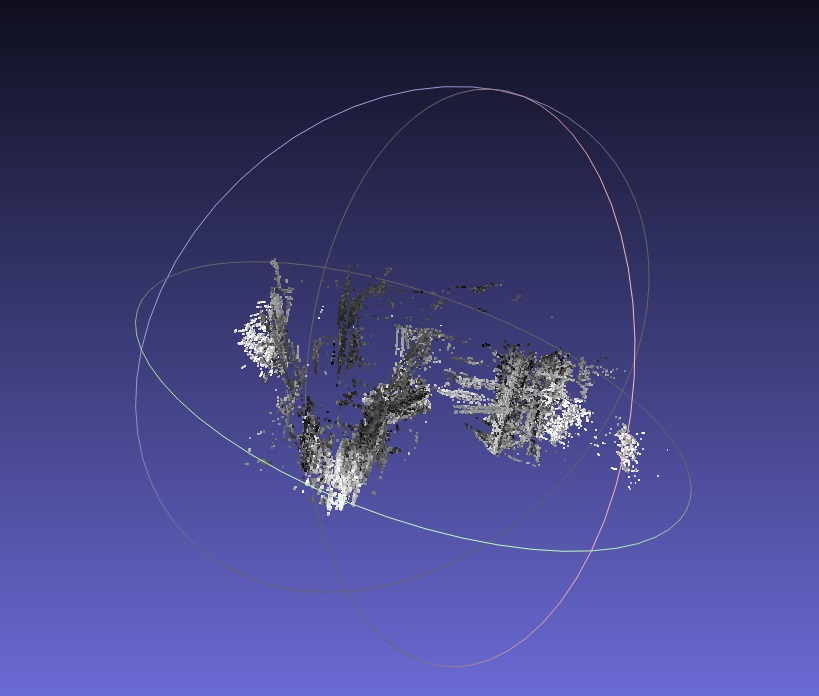
\includegraphics[width= \textwidth]{Imagens/figura4-10.jpg}
	\caption{\textit{Pointcloud} do quintal de uma casa #1}
	\label{fig4:10}
\end{figure}

\begin{figure}[!htb]
	\centering
		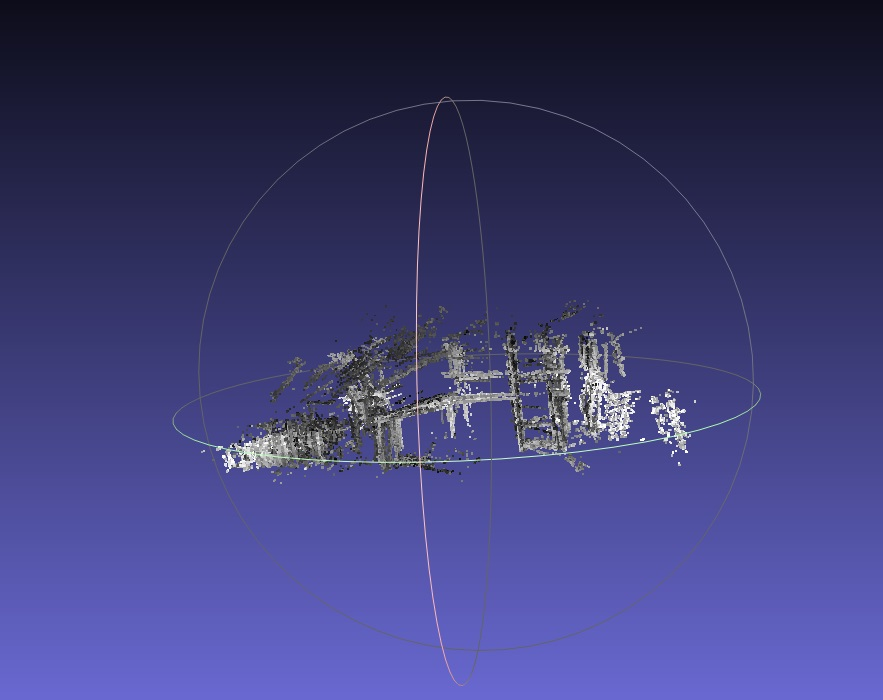
\includegraphics[width= \textwidth]{Imagens/figura4-11.jpg}
	\caption{\textit{Pointcloud} do quintal de uma casa 4.8 #2}
	\label{fig4:11}
\end{figure}

\begin{figure}[!htb]
	\centering
		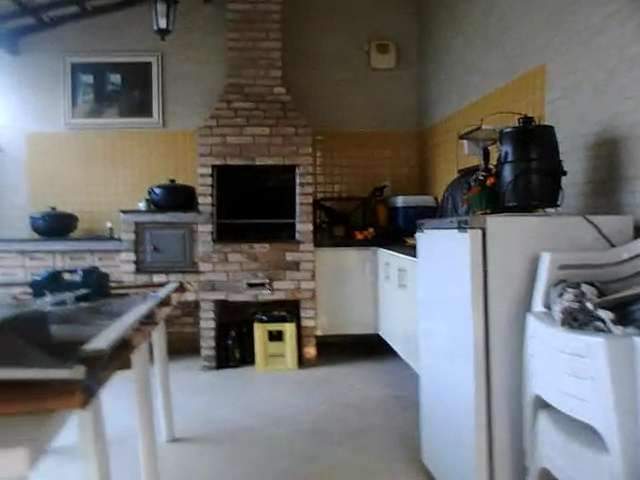
\includegraphics[width= \textwidth]{Imagens/figura4-12.jpg}
	\caption{Fotografia do quintal}
	\label{fig4:12}
\end{figure}


\begin{figure}[!htb]
	\centering
		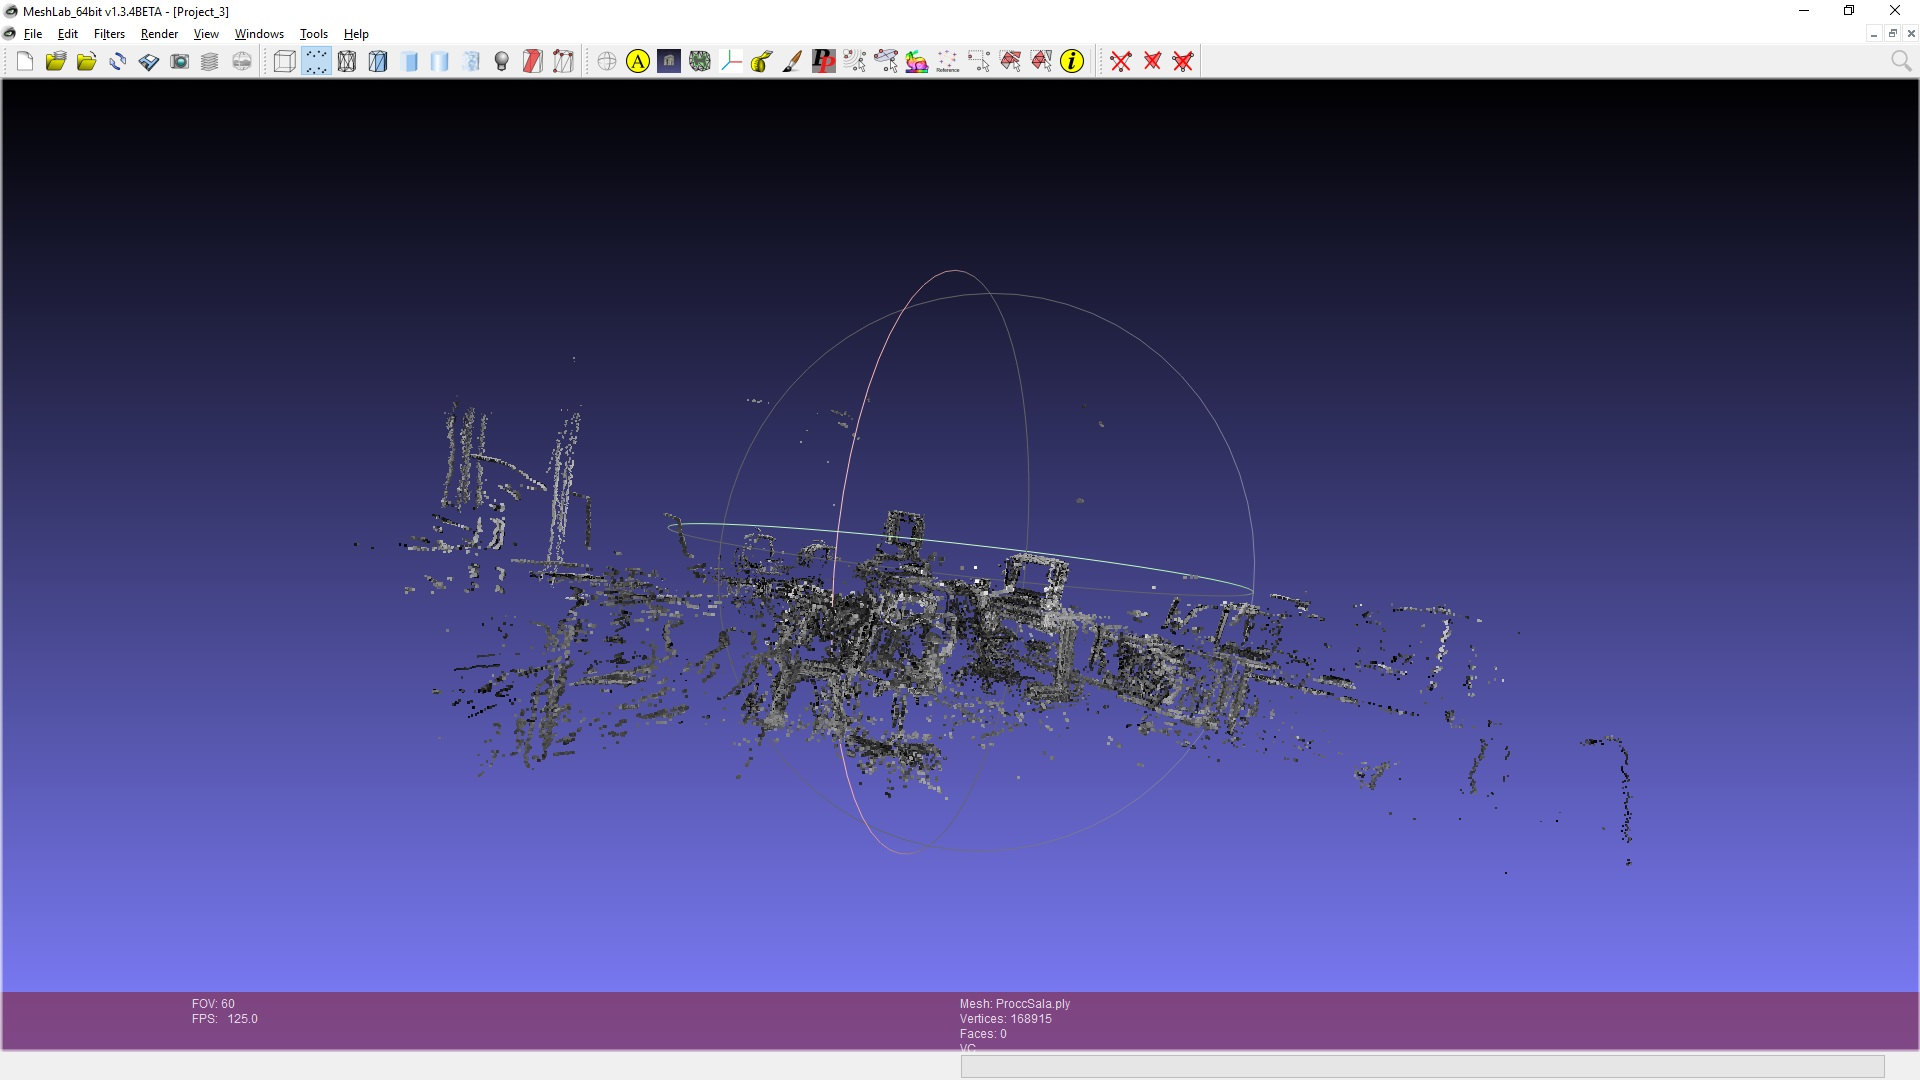
\includegraphics[width= \textwidth]{Imagens/figura4-13.jpg}
	\caption{\textit{Pointcloud} do laboratório de mestrado II #1}
	\label{fig4:13}
\end{figure}

\begin{figure}[!htb]
	\centering
		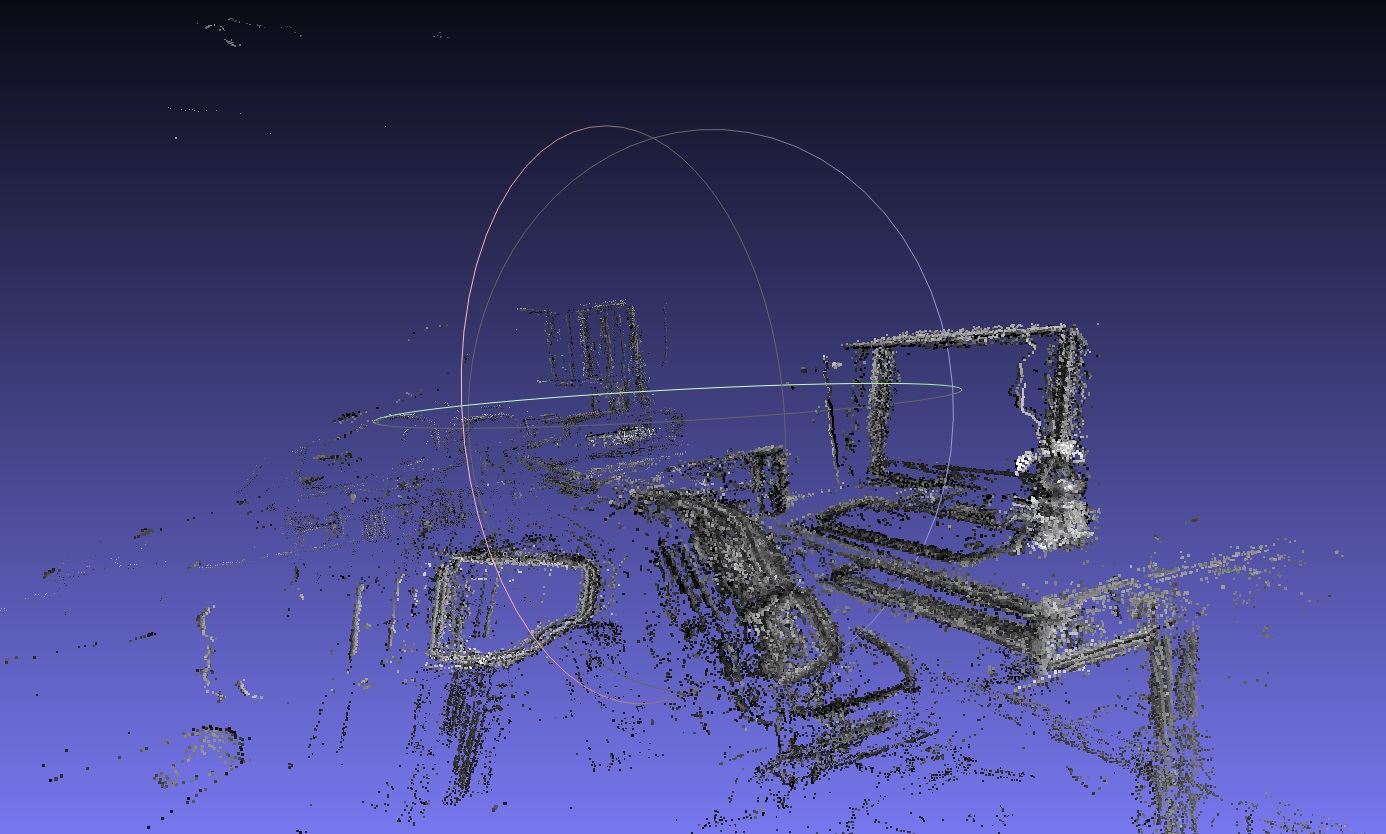
\includegraphics[width= \textwidth]{Imagens/figura4-14.jpg}
	\caption{\textit{Pointcloud} do laboratório de mestrado II #2}
	\label{fig4:14}
\end{figure}

\begin{figure}[!htb]
	\centering
		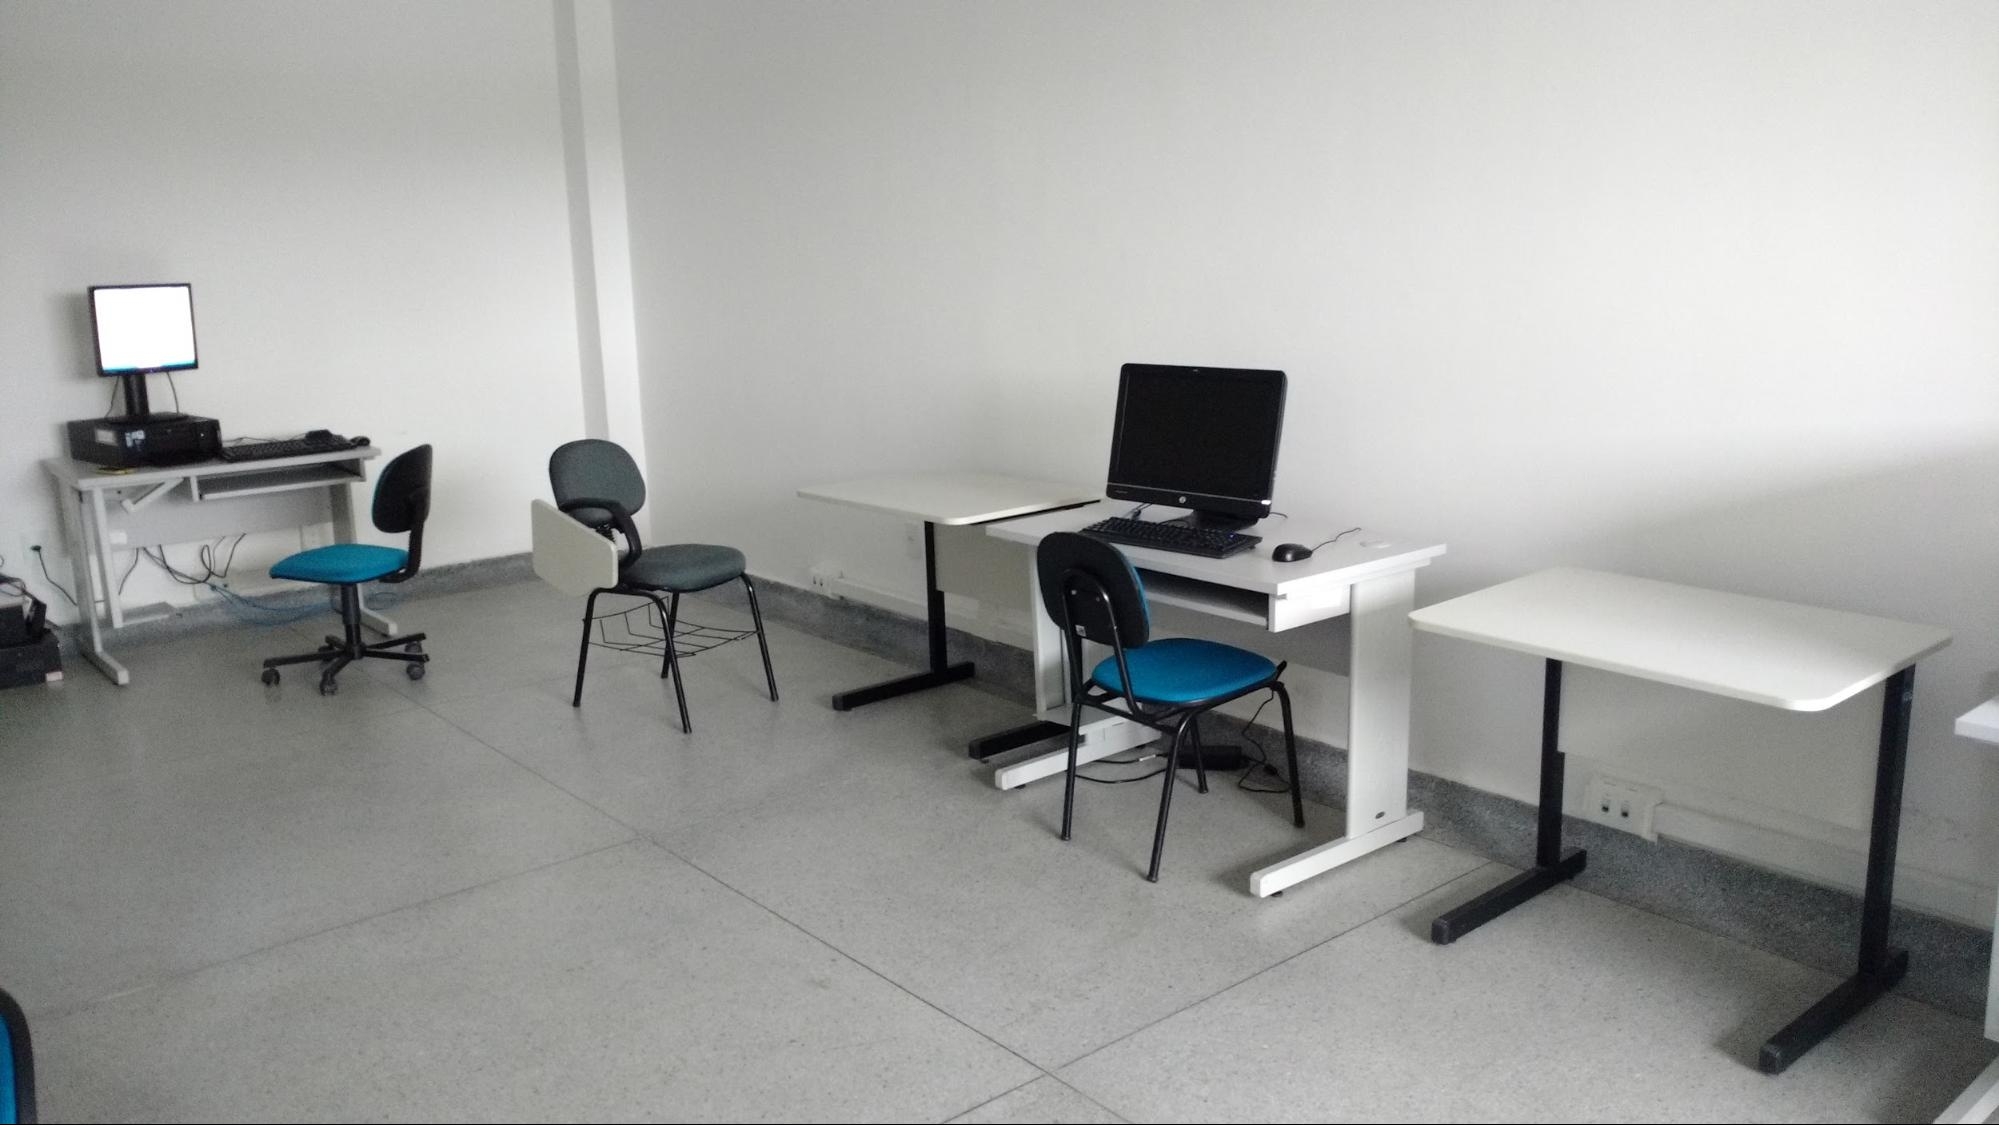
\includegraphics[width= \textwidth]{Imagens/figura4-15.jpg}
	\caption{Fotografia do laboratório de mestrado II}
	\label{fig4:15}
\end{figure}

As imagens mostram as saídas do algoritmo em diferentes ambientes. Percebe-se que apesar de por haver partes incompletos os mapas oferecem uma informação correta se usado de maneira adequada. Em algumas dessas imagens percebe-se que a definição de profundidade foi insatisfatória devido ao meio que foram capturados esses \textit{datasets}, no entanto satisfatória para o intuito original de reconhecimento espacial proposto na introdução.

\section{Problemas}

Alguns problemas encontrados na gravação do \textit{dataset} foram relacionados à luminosidade, que afeta fortemente os quadros capturados, os tornando inválidos para processamento e consequentemente atrapalhando a construção da nuvem de pontos; se tornando mais evidente em ambientes externos sob forte luminosidade ou ambientes internos com pouca luz. A escolha do equipamento também influencia muito, já que inicialmente foi utilizada uma webcam da marca \textit{Logitech}® e frequentemente vários quadros eram encontrados distorcidos, pixelados. Ainda sobre o equipamento, foi notado que a falta de foco também prejudica a reconstrução, dado que o algoritmo não consegue realizar casamentos confiáveis onde um dos quadros está embaçado. As figuras \ref{fig4:16}, \ref{fig4:17} e \ref{fig4:18}  exemplificam alguns casos onde esses problemas ocorreram.

\begin{figure}[!htb]
	\centering
		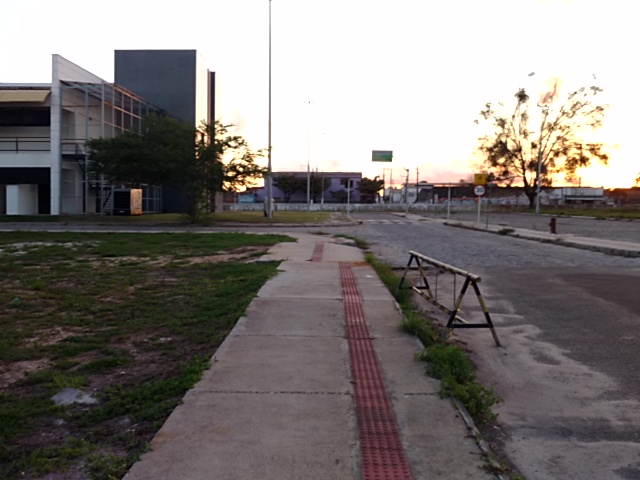
\includegraphics[width= \textwidth]{Imagens/figura4-16.jpg}
	\caption{Fotografia do exterior do prédio do DCOMP, luminosidade não ideal}
	\label{fig4:16}
\end{figure}

\begin{figure}[!htb]
	\centering
		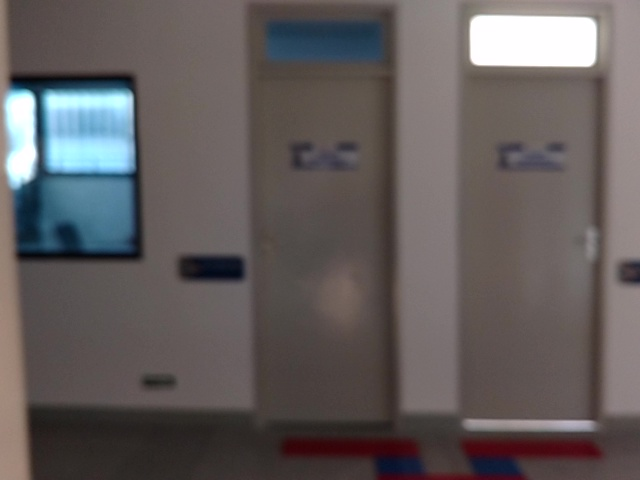
\includegraphics[width= \textwidth]{Imagens/figura4-17.jpg}
	\caption{Fotografia do interior do prédio do DCOMP, pouco foco}
	\label{fig4:17}
\end{figure}

\begin{figure}[!htb]
	\centering
		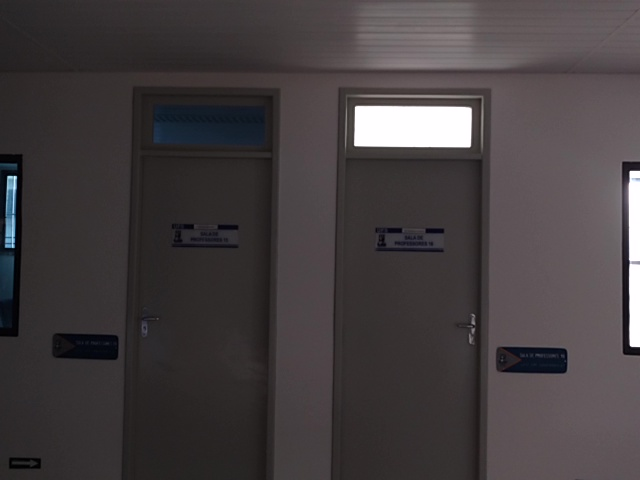
\includegraphics[width= \textwidth]{Imagens/figura4-18.jpg}
	\caption{Fotografia do interior do DCOMP, pouca luminosidade}
	\label{fig4:18}
\end{figure}